\documentclass{article}

% Language setting
% Replace `english' with e.g. `spanish' to change the document language
\usepackage[english]{babel}

% Set page size and margins
% Replace `letterpaper' with`a4paper' for UK/EU standard size
\usepackage[a4paper,top=2cm,bottom=2cm,left=3cm,right=3cm,marginparwidth=1.75cm]{geometry}

% Useful packages
\usepackage{amsmath}
\usepackage{graphicx}
\usepackage[colorlinks=true, allcolors=blue]{hyperref}

%----------------------------------------------------------------------------------------
%
% Title Page: clear and concise
% e.g. technical report title and module code and title, plus your name and student ID number
%
% Abstract Page
%
% Contents Page {shows structure of report - section numbers, heading andpages}
%
% Introduction {very brief description of
%   aims (general) and
%   objectives (what is done to achieve the aims to put report within context/sets the scene for thereader (e.g. where does this development fit within the field);
%               what are theproblems/issues of the subject area}
%
% Body of report {main part of the report; could be divided in several sectionspending the research/discussions you undertake}
%
% Evaluation {evaluate the results; can be a subsection of the Body of report}
%
% Conclusions {condensed version of body; briefly gives key findings andfuture works}
%
% References (Bibliography) {demonstration of your referencing skills}
%
% Appendices {optional, if there is any}
%
%----------------------------------------------------------------------------------------

\title{Your Paper}
\author{You}

\begin{document}
\maketitle

\begin{abstract}
Your abstract.
\end{abstract}

\tableofcontents

% Establish the teritory, the importance and reviewing previous work. how does this assignment relate to cyber-security
\section{Introduction}

Recently in the Harvard Business Review (HBR), \textcite{Milica:2023} identified the challenges regarding cyber-security oversight by company
boards.   In the HBR report survey, boards are saying that they are not seeing eye-to-eye with their CISOs, with one example being that while
\enquote{65\% of board members think their organization is at risk of a material cyber-attack, only 48\% of CISOs share that view.}

European and US companies are spending more each year on cyber-security (having increased over 50\% in the last three years \autocite{Hiscox:2022}),
and that expectation is reflected in the HBR survey, where 87\% of board members are expecting these budgets to increase again in the next year.  

\begin{figure}[!ht] % Single column figure
  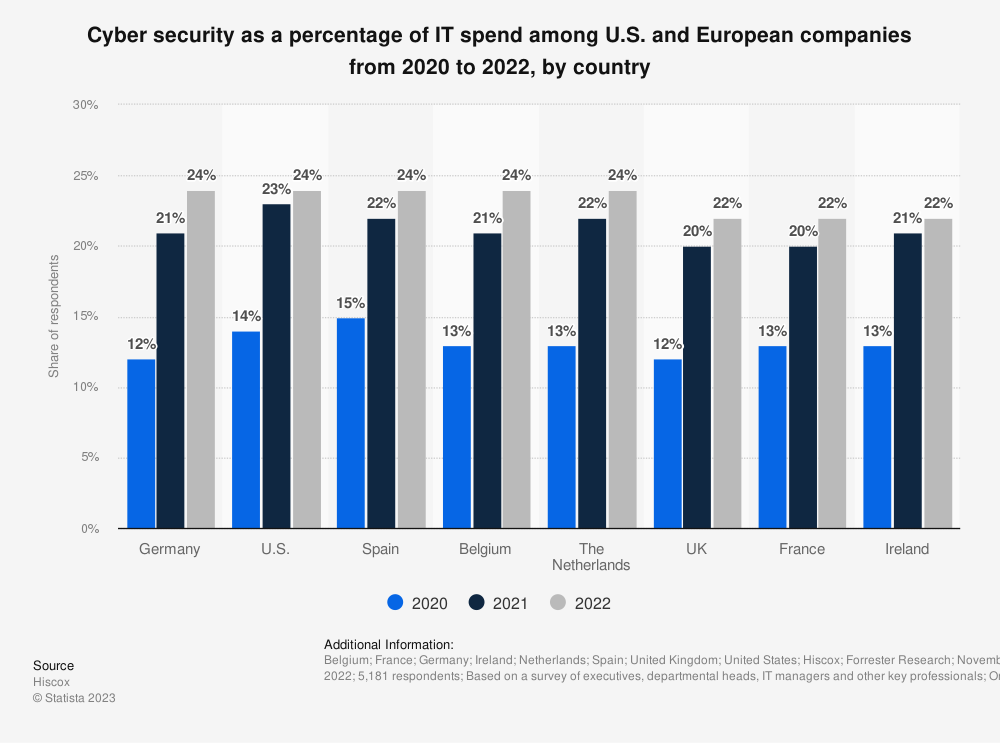
\includegraphics[width=0.95\textwidth]{statistic_id1245356_share-of-it-spend-on-cyber-security-in-the-us-and-europe-2020-2022-by-country.png}\hfill
  \caption{Spending on Cyber Security  \autocite{Hiscox:2022}  Source: Statistica Inc.}
  \label{fig:cybersecurity-spending}
\end{figure}


And the pessimism of the board members' expectations of a material cyber-attack is reflected in the reported monetary damage caused by
cyber-crime, having nearly trebled in the US over the same three-year period \autocite{FBI:2023}.  Yet the HBR reports that 76\% of
board members believe they have made adequate investments in cyber-protection.

\begin{figure}[!ht] % Single column figure
  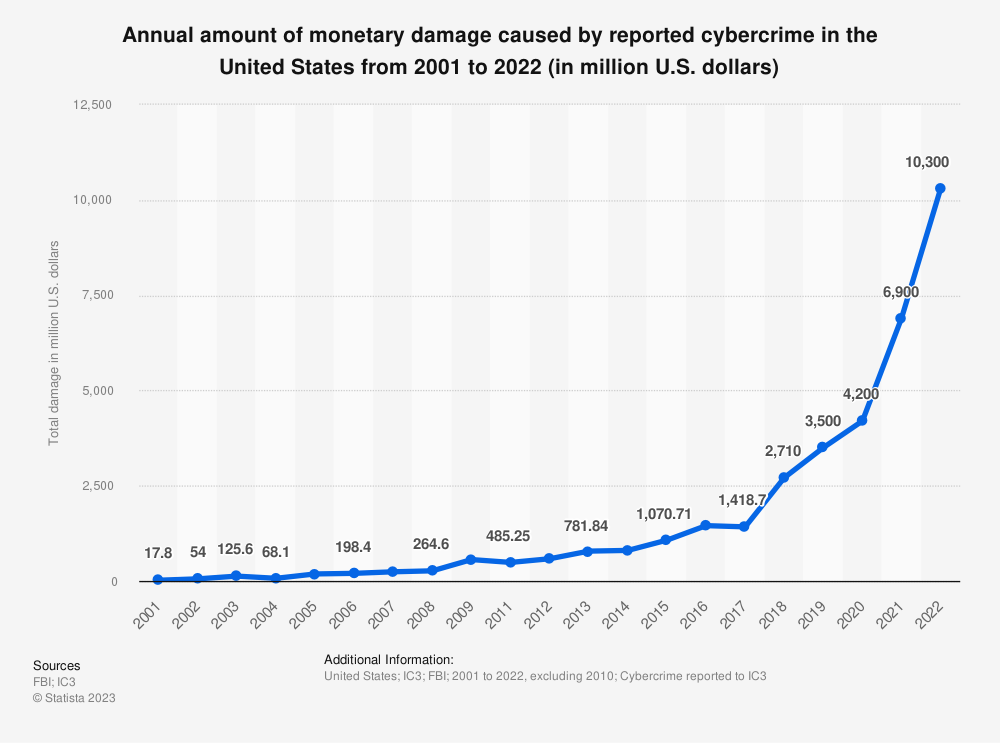
\includegraphics[width=0.95\textwidth]{statistic_id267132_annual-amount-of-financial-damage-caused-by-reported-cybercrime-in-us-2001-2022.png}\hfill
  \caption{Financial Damage caused by Cybercrime in the USA year-on-year \autocite{FBI:2023} Source: Statistica Inc.}
  \label{fig:cybercrime-cost}
\end{figure}

And there lies a key point highlighted by the report; these organisations are talking in terms of protection, not resilience.

% Identify a niche, indicating a gap in in knowledge
\subsection{Resilience vs protection}

The National Institute of Standards and Technology's (NIST) Cybersecurity Framework (CSF) \autocite{NIST:2018} continues to develop a set of baseline
cyber-security practices.  Within this set of functions they outline:

\begin{itemize}
\item Safeguards to ensure the delivery of services [\textit{Protect}].
\item Maintenance of plans to restore services and capabilities impaired due to a cyber-event [\textit{Recovery}].
\end{itemize}
  
Using such a framework it is this reports position that it is possible to engage with this
\enquote{communication gap and board-CISO misalignment [that] hinders progress in cybersecurity}
and to make the improvements to cyber-security oversight highlighted by the HBR authors:

\begin{itemize}
\item Refocus on resilience not protection and address the contradiction between budget expectations and the perceived risk. 
\item Improve communications to ensure cyber-security is continuous priority with ongoing board commitment.
\item Make cyber-security discussions about organisational risk with a strategic imperative, not a technical topic that is difficult to engage with. 
\end{itemize}


%The life of a cyber-security professional can be a thankless task at times.
%Even with cyber-security spend increasing as a percentage of IT
%budgets \autocite{Hiscox:2022}, 

%Considering the challenges identified in the Harvard Business Review article regarding cybersecurity oversight by boards, this report seeks to address these issues and propose a strategic enhancement for Chief Information Security Officers (CISOs). The key concerns include:

%The authors went on to propose a strategic enhancement for Chief Information Security Officers (CISOs).

%\subsection{CISO Challenges in Cybersecurity Oversight by Boards}
%
%\begin{enumerate}
%\item Disconnect Between Boards and CISOs:
%     \begin{itemize}
%        \item Limited alignment between boards and CISOs.
%        \item Insufficient interaction hindering meaningful cybersecurity discussions.
%        \item Communication gaps and misalignment impeding progress in cybersecurity.
%     \end{itemize} 
%\item Focus on Protection Over Resilience:
%     \begin{itemize}
%        \item Boards prioritizing cyber protection despite a high perceived risk.
%        \item Investments in protection not directed to critical areas.
%        \item Advocacy for a shift towards organizational resilience.
%     \end{itemize} 
%\item Cybersecurity as a Technical Topic:
%     \begin{itemize}
%        \item Boards viewing cybersecurity primarily as a technical issue.
%        \item Limited time in board meetings making it challenging to address nuances.
%        \item Need for a shift from technical to management challenges in discussions.
%     \end{itemize}
%\item Board Composition and Expertise:
%     \begin{itemize}
%        \item Many boards lacking cybersecurity expertise.
%        \item SEC proposing explicit cybersecurity recommendations for boards.
%        \item Necessity for board composition changes to incorporate cybersecurity knowledge.
%     \end{itemize} 
%\item Priority and Commitment:
%     \begin{itemize}
%        \item A quarter of boardrooms not viewing cybersecurity as a priority.
%        \item Inadequate frequency of cybersecurity discussions.
%        \item The necessity of making cybersecurity a continuous priority with ongoing commitment.
%     \end{itemize}
%\end{enumerate}

%Organisations are clearly spending more on cyber-security.  Financial damage is going up. But the HBR report highlights a focus on prevention rather than resiliency.  
   
%\subsection{The CISO and current state of malware attacks on Windows.}

%\textbf{Importance of addressing issues in cybersecurity oversight by boards}.

%To address these challenges, this report proposes a strategic proposition aimed at enhancing the CISO's position within the organization. The proposition includes:
%\begin{enumerate}
%      \item Engagement with Senior Executives:
%         \begin{itemize}
%            \item Demonstrating the importance of cybersecurity as an organizational imperative.
%            \item Building personal relationships with senior executives to bridge the communication gap.
%         \end{itemize}
%      \item Explanation of Cyber-Resilience Program:
%         \begin{itemize}
%            \item Clearly communicating the organization's cyber-resilience strategy.
%            \item Translating technical jargon into business language for better understanding by the board.
%         \end{itemize}
%      \item Initiatives within the Department:
%         \begin{itemize}
%            \item Developing regular cybersecurity reports to provide transparent insights.
%            \item Showcasing the department's efforts in enhancing cyber resilience.
%         \end{itemize}    
%      \item Use Case Report on Process Injection Attacks:
%         \begin{itemize}
%            \item Presenting a real-world use case demonstrating new process injection attacks.
%            \item Evaluating the effectiveness of the organization's Endpoint Detection Response system (EDR).
%         \end{itemize}         
%      \item Ensuring EDR Vendor Adaptation:
%         \begin{itemize}
%            \item Using the use case report to ensure the EDR vendor is adapting to new threats.
%            \item Strengthening the organization's defence mechanisms against evolving cyber threats.
%         \end{itemize}
%\end{enumerate}


%This comprehensive approach aims not only to address the challenges outlined in the Harvard Business Review article but also to elevate the CISO's role by fostering better understanding, engagement, and preparedness within the organization. cite \href{https://www.cisa.gov/cross-sector-cybersecurity-performance-goals}{cross-sector-cybersecurity-performance-goals} and 



%Relying on EDR systems as a principle defence against a myriad of attacks alieviates many problems.  But it does not alievate the communication gap between company boards
%and the cyber and information security professionals that protect their organisation.  CISOs need to understand the threat landscape, their mitigants to attacks, and
%where failures in their own security systems may fail.  Having new internal analysis and being fully abreast of the threats, vulnerabilities and mitigants of their
%systems will equip our CISO with the information they need to formulate and communicate a set of action/response readiness to the senior executives and board members.
%\subsection{Introducing Mockingjay: Importance of understanding process injection techniques.}
%This cat-and-mouse game beween security groups on the one hand, and the evasion and increased sophistication and novelty on the part of malicious actors on% the other \ldots
%\textit{introduce EDR} \ldots
%For vendors of EDR, MDR \& XDR solutions investigating existing and emerging threats is an on-going process \href{https://research.tue.nl/files/305661196/Olteanu_I.C..pdf}{evaluating the response effectiveness of their XDR technology}.

% Occupy the niche; purpose of new research, listing questions, the value of the work and the structure of the writing


\subsection{Turning a threat into a strategic enhancement for the CISO}

This paper presents a model for the type of analysis that a CISO should be requesting from their information security teams.

Process Injection (PI) is a technique to dynamically modify a running process to introduce some new functionality.  It is used by malware and virus coders to
deliver, and execute, a malicious payload into the addressable memory space of a legitimate process.  This is engineered to be done without
being detected by anti-virus software or other defensive systems. 

End-point Detection and Response (EDR) is an integrated security solution that uses real-time continuous monitoring of processes and systems, and the data generated from these systems, to detect malware either directly, or through anomalous behaviour of the monitored systems.

This paper reports on a new process injection technique named ``Mockingjay'' \autocite{Peixoto:2023} that seeks to evade the protections offered by EDR technologies.  We will investigate the attack in a case study produced by a cyber-security group in a hypothetical organisation and couch the response
to address all NIST CSF functions and include resilience as a core part of the response to the threat.

%, and specifically with behaviours that could be used to detect API attacks \autocite{Wang:2022}.

%We will analyse the ``Mockingjay'' attack and identify the defences offered by modern XDR systems and ask if there's a credible chance of evading detection.  By looking at an implementation of the attack we will ask in what ways a threat detection system strengthen it's defences, and what artifacts could be automatically produced that could demonstrate any anomoly in a systems behaviour. 

Section 2 is a overview of changing landscape of threat actors and defence mitigants.  We review process injection methods, focusing in on file-less exploits leveraging the Windows system used by Mockingjay.  We also look at how malware detection has adapted to these threats and examine end-point protection such as EDRs.

%We will then look at methods a identifying these attacks and look at the likelihood of Endpoint Security products of identifying the attack.   An investigation into the Mockingjay attack and against a recently published paper ``Procguard'' \autocite{Wang:2022} and asks whether this attack method would lickly be caught.

Section 3 is the case study on the Mockingjay process injection attack that a CISO should be expecting from their team.  It will demonstrate that
every analysis that the cyber-security team undertakes can be an opportunity to safeguard critical services and ensure that services can be
restored from as successful attack.

%crystalise challenges
%that our titular CISO should be engaging his vendor on.  It should also feed back into the cyber-security playbooks that the organisation has, and
%the threat and response reported back to senior executives and boards.

%to use reinforcement to identify ``RWX'' code injections that should be part of a corporations EDR solution.
% {jwang,mcj123,ZiangLi,2018302180148,iwangjye}@whu.edu.cn

%Section 5 is an implementation of the attack and will look at manually identifying an infected process and generating artifacts that could be used in automating the process.

Section 4 is an evaluation section, reflecting on the project.

Section 5 is the conclusion where we highlight how taking a holistic view when understanding threats and threat actors can help build more
resilient cyber-security systems and define the CISO function as an important strategic foundation for mitigating operational risks.

%and will suggest risks and mitigants for process injection attacks and further research that could be undertaken to adapt to and mitigate evolving cyber-security threats.


% Section 2 is a literature review of HBCI methods and endpoint security that is typically relied upon to prevent these types of attack. We will then look at methods a identifying these attacks and look at the likelihood of Endpoint Security products of identifying the attack.

% Outline

% introduce EDRs and how they are used to protect organisations

% introduce process injection attacks: MITRE, and NT process attacks

% how do EDRs

%\section{Proess Injection Attack and EDR Repsonse Primer}
\pagebreak
\section{The evolving threat landscape of process injection}

Malware attacks using code injection predates modern Windows operating systems, with the first notorious example probably being the ``Moris Worm''
that targeted UNIX systems in 1988, by exploiting a buffer overflow bug \autocite{Spafford:1989}.  This remote exploit has several
traits that malware writers still try to find; it executes at the privilege level of the service being attacked and there is no complicated
thread execution needed to initiate.

The history of the code injection techniques used by Windows malware could be argued to have started with more altruisic motives.
Microsoft themselves patented a method to map an external module into a target process in 2004 \autocite{Ghizzoni:2004}.  This has the
stated aim of, somewhat ironically supporting applications such as ``anti-virus programs, profilers, debuggers, and pseudo-localization testing''.

And the race was then on to determine whether a program utilising these dynamic-link library (DLL) loading methods were malicious.
The first malicious code detection methods would judge the motives by looking at static evidence within the program file itself,
with checks based on code signing, file metadata, Portable Executable (PE) file header analysis, etc. \autocite{Jang:2007}.

\subsection{Code Injection Taxonomy}

To understanding the general principles it is helpful to use the taxonomy of \textcite{Barabosch:2014}.
The authors distinguish between Host-Based Code Injection Attacks (HBCIA) that orginate and infect process on the
same system from Remote-Based Code Injection Attacks (RBCIA), such as worms, where the victim process is on a system
remote from the infecting agent.

They then neatly summarise the HBCIA into three steps that we will see when we meet Mockingjay:

\begin{enumerate}
\item selecting a victim process,
\item copying code into the victim process, and
\item executing the injected code.
\end{enumerate}

\begin{figure}[ht]
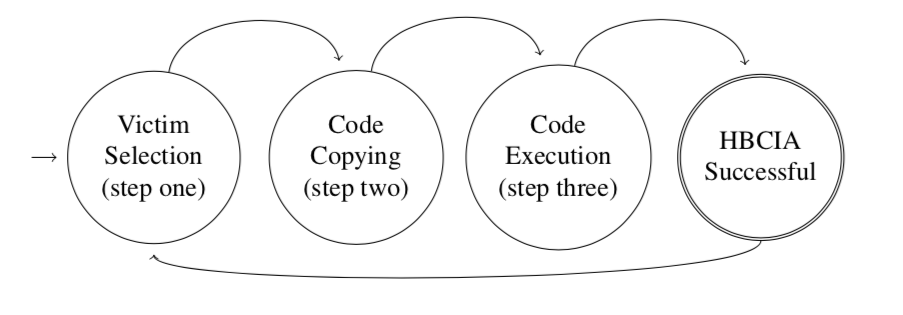
\includegraphics[scale=0.4]{hbcia_3step_algo.png}
\caption{HBCIA Attack Steps \autocite{Barabosch:2014}}
\end{figure}


How we select our victim and how we execute our code can be categorised to aid our understanding of attack methods as:

\begin{itemize}
\item Victim Selection:
  \begin{enumerate}
  \item Targeted Injection:
    \begin{itemize}
    \item Malware selects a specific subset of processes to inject into based on an internal target list (e.g. critical
        processes like explorer.exe.)
    \item Less suspicious as avoids risky/unnecessary processes.
    \end{itemize}
  \item Shotgun Injection:
    \begin{itemize}
    \item Greedy approach that blindly injects itself into as many accessible processes as possible.
    \item More suspicious as may accidentally target antivirus or risky processes.
    \end{itemize}
  \end{enumerate}
\item Code Execution:
  \begin{enumerate}
  \item Concurrent Execution:
    \begin{itemize}
    \item The injected code runs in parallel with the original code in the victim process, with original process continue executing.
    \item Additional threads are spawned for the injected code.
    \end{itemize}
  \item Thread Manipulation:
    \begin{itemize}
    \item The injected code replaces or blocks the original victim process's thread(s) which do not continue.
    \item Victim process exhibits mainly the injected code's behavior.
    \end{itemize}
  \end{enumerate}
\end{itemize}

\begin{table}[!ht]
  \centering
  \caption{Prevalence of classes of HBCIA algorithms \autocite{Barabosch:2014}}
\begin{tabular}{ |p{2cm}|p{2cm}||p{3.8cm}|p{3.8cm}|  }
  \hline
  & & \multicolumn{2}{|c|}{Victim Selection} \\
  \cline{3-4}
  & & Targeted Injection & Shotgun Injection \\ 
  \hline
  \hline
  Code  & 	Concurrent  & TICE 58\% & SICE 23\% \\
  Execution & Execution &  Hanthie (Linux) & Flashback (Mac OS X) \\
  \cline{2-4}
  &  Thread  & TITM 20\%  & SITM: 00\% \\
  & Manipulation & Stuxnet (Windows) &  \\
  \hline
\end{tabular}
\label{table: HBCIA}
\end{table}


\subsection{Common techniques in windows malware attacks}

When understanding the possible approaches to protecting against code injection attacks researchers look at all classes of attacks.
MITRE ATT\&CK(R) is a knowledge base of advesary tactics which is a useful resource and collects information on injection implementations
for all major OSs, with a dizzing array of samples \autocite{Mitre:2017}.

A more useful summary when understanding the Mockingjay attack is to look at the common Windows techniques \autocite{Hosseini:2017}.  We
can follow a line of evolution in newer attacks, from the classic DLL injection method, to file-less methods, and newer methods that
avoid telltail behaviours of older techniques.

\begin{table}[!ht]
\centering
\caption{10 Windows Process Injection Techniques \autocite{Hosseini:2017}}
\begin{tabular}{ |p{3.5cm}||p{10.5cm}|  }
  \hline
  \multicolumn{2}{|c|}{Ten process injection techniques} \\
  \hline
  Name & Description \\
  \hline
  Classic DLL Injection Via Createremotethread And Load Library
             & The malware writes the path to its malicious DLL in the virtual address space of another process,
               and ensures the remote process loads it by creating a remote thread in the target process. \\
  \hline
  PE Injection
             & Copy malicious code into an existing open process and cause it to execute (either via a
               small shellcode, or by calling CreateRemoteThread). The malware is file-less, not placing a malicious DLL
               on the disk.  It still allocates memory in a host process (e.g. VirtualAllocEx),
               but writes its malicious code by calling WriteProcessMemory. \\
  \hline
  Process Hollowing (A.K.A Process Replacement and Runpe)
             & The malware unmaps (hollows out) the legitimate code from memory of the target process, and
               overwrites the memory space of the target process (e.g., svchost.exe) with a malicious executable.\\
  \hline
  Thread Execution Hijacking A.K.A Suspend Inject and Resume (SIR)
             & After getting a handle to the target thread, the malware puts the thread into suspended mode by
               calling SuspendThread to perform its injection. The malware calls VirtualAllocEx and
               WriteProcessMemory to allocate memory and perform the code injection. Targeting an existing thread
               of a process, during analysis you will probably see calls to CreateToolhelp32Snapshot and
               Thread32First followed by OpenThread. \\
  \hline
  Hook Injection via Setwindowshookex
             & Malicious DLL loaded upon an event getting triggered in a specific thread. This is usually
               done by calling SetWindowsHookEx to install a hook. \\
  \hline
  Injection and Persistence via Registry Modification (E.G. Appinit\_DLLS, AppCertDLLs, IFEO)
             & Appinit\_DLL, AppCertDlls, and IFEO (Image File Execution Options) are all registry keys that
               malware uses for both injection and persistence. \\
  \hline
  APC Injection And Atombombing
             & Use APC to force another thread to execute their custom code by attaching it to the APC
               Queue of the target thread. \\
  \hline
  Extra Window Memory Injection (EWMI) via Setwindowlong
             & Injecting into Explorer tray window’s extra window memory, and has been used a few times
               among malware families such as Gapz and PowerLoader. There is not much room in EWM, so the
               malware writes code into a shared section of explorer.exe, and uses SetWindowLong and
               SendNotifyMessage to have a function pointer to point to the shellcode, and then execute it. \\
  \hline
  Injection Using Shims
             & Shims allow developers to apply fixes to their programs without the need of rewriting code.
               Malware can take advantage of shims to target an executable for both persistence and injection.
               Windows runs the Shim Engine when it loads a binary to check for shimming databases in order
              to apply the appropriate fixes. \\
  \hline
  At Hooking and Inline Hooking (A.K.A Userland Rootkits)
            & Malware changes the import address table. When a legitimate application calls an API located
              in a DLL, the replaced function is executed instead of the original one. \\
  \iffalse
\fi
  \hline
\end{tabular}
\label{table: ProcessInjectionTechniques}
\end{table}


\subsection{Endpoint security}

EDR solutions cover a wide range of cyber-security capabilities to monitor in real time the health of applications
and services, detect anomolous activity and respond to an attack.
Related technologies are Managed Detection and Response (MDR) \autocite{Hayes}, which offers endpoint security as a service, and
eXtended Detection and Response, which consolidates applications and collects data from across the enterprise to
have a wider scope of view to detect changes in behaviours across systems.

For the rest of this report we will not delve into the specifics of the capabilities of the various end-point
solutions.
But we can use the MITRE categories to see where these defences are focused:


\begin{table}[!ht]
  \centering
  \caption{Attack Mitigants \autocite{Mitre:2017}}
\begin{tabular}{ |p{1.2cm}||p{2cm}|p{11.5cm}|  }
  \hline
  \multicolumn{3}{|c|}{PI Mitigation List} \\
  \hline
  ID	& Mitigation & Description \\
  \hline
  M1040	& Behavior Prevention on Endpoint &	Endpoint security solutions can be configured to block some types of
                                            process injection attacls by monitoring certain API calls
                                            and observing telltail sequences of behavior that occur during the
                                            injection process.  Attack Surface Reduction (ASR)
                                            rules may prevent Office applications from code injection.\\
  \hline
  M1026 & Privileged Account Management	& Restrict the use of certain applications that can be abused by
                                          process injection to privileged users only. Apply and monitor: advanced access control and
                                          process restrictions. \\
  \hline
\end{tabular}
\label{table: Mitigations}
\end{table}


\subsection{Deploying a file-less payload into Windows memory space}

The Nirvana callback is a method Microsoft developed to control a running process with needing to recomplie or rebuild code.
It inserts a user mode function to be called on the return from a kernel system call.
Originally developed as a legitimate instrumentation technique,
it is important to our discussion as it has been used to allow malware payloads to be delivered directly into the
address space of a running process \autocite{Dequeker:2023}.

An attacker loads a payload into the RWX section then registers a Nirvana callback to execute the call after the normal program
execution makes a system call.

\begin{figure}[ht]
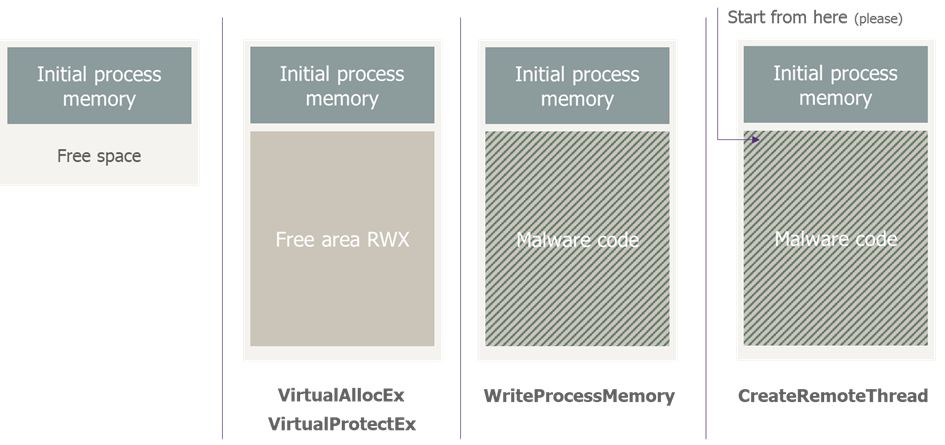
\includegraphics[scale=0.9]{dequeker_standard_process_injection_pattern.png}
\caption{RWX process Injection pattern \autocite{Dequeker:2023}}
\end{figure}
 
The direct attack can be detected by an EDR/XDR as it needs to use monitored NtSetInformationProcess call.  But the pattern
will be adapted by Mockingjay.

%\subsection{Use cases for process injection in malware}

%\subsubsection{Evading detection}

%\subsubsection{Privilege escalation}

%\subsubsection{Payload delivery and execution}

%\subsubsection{Deploying Payload into Windows Memory Space}

% \href{https://modexp.wordpress.com/2018/07/15/process-injection-sharing-payload/}{Process injection sharing payload}


%\autocite{Zhan:2018}

%\href{https://www.riskinsight-wavestone.com/en/2023/10/process-injection-using-ntsetinformationprocess/}{PI using NTSetInformationProcess}

%\href{https://github.com/elddy/Windows-NTAPI-Injector}{NTAPI injector} 

%\href{https://gist.github.com/WKL-Sec/96e17188e4c159c2cdf7ff2c111130cc#file-local-c}{Injector examples in C}

%\href{https://www.unknowncheats.me/forum/anti-cheat-bypass/286274-internal-detection-vectors-bypass.html}{internal detection vectors bypass}

%\href{https://medium.com/@s12deff/process-injection-with-random-rwx-memory-spaces-3e3651149527}{PI with random RWX memory spaces}


%\subsection{Detection and Mitigation}

%\subsubsection{Current strategies for detecting process injection}

%\subsubsection{Anti-malware tools and techniques}

%\subsubsection{Best practices for preventing and mitigating process injection attacks}

%\begin{itemize}
%\item DLL Injection
%\item Code Injection
%\item Atom Bombing
%\item Reflective DLL Injection
%\end{itemize}


\subsection{EDRs response to an evolving threat landscape}

EDR/XDR cyber-security solutions have been incorporating protections of increasing levels of sophistication.

At the first level, as discussed earlier, there are static monitoring of a specific machine DLLs and processes to detect changes.

Making sure that certain subsystems have not been modified, had elevated permissions, or unknown processes running on the monitored system.

Next, user and entity behaviour analytics (EUBA) tools identify changes in behaviours that could indicate a threat.  This could include the
applications and systems a user normally uses, looking for configuration changes, and scanning log files for changes in behaviour.

Statistical modeling will profile normal activity and continuous monitoring will attempt to descern anomolous behaviour as a threat occurs.

Researchers are now looing to detect process injection using fine-grained analysis of API call chains using deep learning \autocite{Wang:2022}.

Anomaly detection can be prone to false positives.  The threat actor will look for attacks that could look like innocent behavior.

The response is to use increasingly sophisticated AI and machine learning techniques by looking at system entity interactions.
An example of this a paper by \textcite{Zengy:2022} where providence analysis of system auditing records seeks to search for anomolies
that attacks produce.

We can see a series of adaption and evasion moves that leaves total cyber-protection and ideal that can not be always realised. 


%End-point Detection and Response Systems (EDR) have developed to counter these myriad threats.  These systems are gaining in sophistication and adversaries
%are on the hunt for new ways to evade these systems.

%In this report we look at a new variation of one attack technique, process injection, and ask how EDRs protect against these attacks and how
%this new technique would evade those barriers.  In particular we are looking at the ``Mockingjay'' attach that targets modern Windows machines.

%These protections can be signatu


% \href{https://www.crowdstrike.com/cybersecurity-101/endpoint-security/edr-vs-mdr-vs-xdr/}{EDR vs MDR vs XDR}
%HBCI techniques work on injecting code into running processes and having that code executed as part of the normal process
%execution.  End-point Detection and Response (EDR) systems \autocite{Hayes:2023} provides realtime visibiluty

%Process injection seeks bypass EDR hooks by injecting code into trusted processes with RWX permissions already set.

%\subsection{Emerging trends in malware attacks on Windows}

%\subsection{Advancements in process injection techniques}

%\subsection{Future predictions for the evolution of these threats}





% Section 3 an investigation into the Mockingjay attack and against a recently published paper ``Procguard''  and asks whether this attack method would lickly be caught.
\section{Case Study: Introducing the MockingJay Process Injection Attacks}

In our review of one technique used by malware groups, we now ask how a CISO in a modern organisation can stay ahead of the curve,
have an realistic appraisal of the threats their organisation might face, and develop a resilient cybersecurity infrastructure.

Our hyperthetical CISO has been active in putting in place an XDR system that has reduced manual processes to patch individual cybersecurity
applications, leveraged the vendor's expertise to configure the monitoring of data across endpoints, servers, cloud networks and Security
information and event management (SEIM) systems.

Our enlightened CISO has empowered his team team to research ways to improve cybersecurity, and looks foward to using their insights to engage with
senior stakeholds within the organisation, and to regularly brief the board on operation risks and mitigation plans.  

One of the team security engineers has come across a new potential exploit and has asked to produce this case study for the CISO and his team.  The
Mockingjay attack \autocite{Peixoto:2023} is a real and novel process injection attack created by Security Joes, a
``multi-layered MDR \& incident response company'' based in Tel Aviv.

\subsection{Introduction}


\textbf{Key Problems}:

\begin{enumerate}
\item A new process injection attack has been identified by Securities Joe.  The exploit circumvents the allocation
  and permission APIs that most EDR systems monitor.  It  does this by using existing RWX code sections without invoking
  new threads.
\item Our systems may be vulnerable to this attack which could allow a Windows executable to self injection or remote injection.
\item Recently Citrix has reported vulnerabilities in their NetScaler Application Delivery Controller (ADC) and Gateway products that
  could allow:
  \begin{itemize}
  \item \citetitle{CVE-2023-3467} \autocite{CVE-2023-3467}.
  \item \citetitle{CVE-2023-3519} \autocite{CVE-2023-3519}.
  \item \citetitle{CVE-2023-4966} \autocite{CVE-2023-4966}.
  \end{itemize}
\item The Cybersecurity and Infrastructure Security Agency (CISA) has reported that the malware group LockBit \autocite{CISA:2023a} has
  been found to be actively exploiting CVE-2023-4966 to obtain initial access to Boeing Distribution Inc. \autocite{CISA:2023b}.
\end{enumerate}

Our organisation should be prepared for similar attacks and group should review our cyber-defences in light of this information.
As always, we should seek to prevent any successful attack, but also improve our cyber-resilience in the face of a sucessful breach.

This case study will:
\begin{enumerate}
\item Review the salient points of the new attack vector, how it may evade our XDR system and how we may identify an attack.
\item Understand ransomware threat actors such as LockBit and how we can detect and respond to ransomware.
\item Prepare a set of recommendations in line with our Cyber-Security Framework (CSF) \autocite{NIST:2018}.
\end{enumerate}


%\subsection{Real-world examples of malware employing process injection on Windows}
\subsection{Context: Detailed Analysis of New Process Injection Attack}

Attackers could exploit the Mockingjay technique to circumvent XDR process monitoring and anti-virus sofware by avoiding
common system API calls used by malware.  

The security report was able to demonstrate:

\begin{enumerate}
\item Self-injection
\item Remote process injection: injected a shellcode into `ssh.exe` in the
\end{enumerate}

\subsection{Alternatives: How Attack could Evade XDR}

The first line of our defense of an attack based on the Mockingjay process injection technique will be our XDR system.

Using `Lifecycle of a Ransomeware Incident` produced by \autocite{Certnz:2021} and the modus-operandi of the LockBit
group \autocite{CISA:2023}, we should anticipate:

\begin{enumerate}
\item Direct attack through our application gateway (Intenet-exposed Service).
\item Phishing attack through email.
\end{enumerate}

If either of these two approaches are successful, 

\begin{figure}[ht]
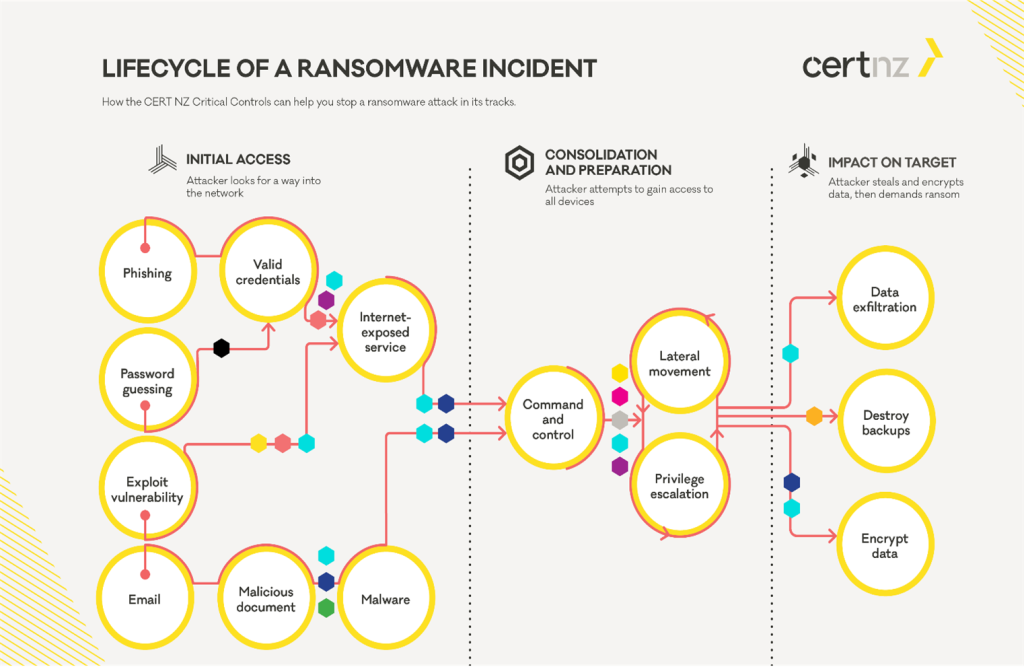
\includegraphics[scale=0.55]{certnz_aa23-165a.png}
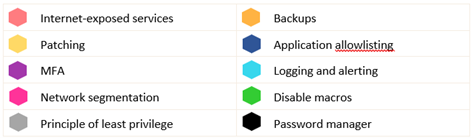
\includegraphics[scale=0.6]{certnz_aa23-165b.png}
\caption{Ransomeware Layered Mitigations \autocite{Certnz:2021}}
\end{figure}

\pagebreak

%\subsection{Analysis of the impact and consequences of these incidents}
\subsection{Proposed Solution: Assessing and Improving Cybersecurity Measures}

As Security Joes is a security system vendor, the report itself lists a number of ways that the attack could be detected. At
the first instance, we should be talking to our XDR vendor to ensure we have the functionality to automate these steps.  At
the very least we need to be able to perform ad-hoc scans across our infrastructure and windows systems to flag the following:

\begin{enumerate}
  \item point a:
\end{enumerate}


\subsection{Recommendations}

Our organisation is committed to the continud review of new attacks and actively researches the possible impact of reported attacks.
This active engagement with the cybersecurity community and our vendors allows us to adapt quickly to changes in the threat landscape.

For this case study, we recommend the following actions under each of the NIST CSF fuctions:

\begin{itemize}
\item Identify: Ensure all systems are patched for the CVEs identified and engage with our XDR vendor to respond to this new threat.
\item Protect: review XDR solutions are monitoring log files to detect encryption; use technique to find vulnerable exes and block them (eg. visual studio ssh exfiltration block known malicios systes
\item Detect: Develop a Mockingjay red-team exercise against our XDR; test for the detection of the loading of NTDLL.dll from disk.
\item Respond: Ensure that our organisation is able to report to all relevant authorities  and abide to our legal responsibilities for disclosuress
\item Recover: review perform disaster recover tests to restore systems from backups and that backups are immutable 
\end{itemize}







% VII. Legal and Ethical Considerations
% A. Legal implications of malware attacks and process injection
% B. Ethical considerations in combating malware
% C. Collaborative efforts in law enforcement and cybersecurity


% Section 4 is an implementation of the attack and will look at manually identifying an infected process and generating artifacts that could be used in automating the process.
%\section{So Hard Hard is this Anyway?  Attack!}

Description of implementation, etc

\begin{listing}[!ht]
\inputminted{c++}{tex/code/mockingjay.cpp}
\caption{Mockingjay Implementation C++ code}
\label{listing:1}
\end{listing}

\subsection{Inoculation: Generating artifacts}

Blah....



\section{Reflection}


This report looks holistically at the threat landscape and cyber-security teams in an organisation following on from points raised by HBR report. 

Looking in depth a one element of cyber-security defences, produced in the case study, the breadth of the topic I would need to summarise, as
background became apparent.  Also, the difficulty of providing a review of end-point cyber-protection also became apparent. 
  
Overall, making this a higher-level discussion on the benefits of resilience over protection made a better topic for this unit, and I am happy
with where the report is pitched and think I have achieved that objective. 

What I have not been so successful in is encapsulating the technical knowledge of Windows process injection and detect methods needed to
support the case study and present that in a way that is congruent with the higher-level focus of the overall report.

On balance, I believe I have achieved the stated aims of the report and that the technical details correct.  For this I would expect a distinction grade.


\section{Conclusion}

\begin{itemize}
   \item Recap of key points related to malware attacks and process injection on Windows
   \item Call to action for cybersecurity professionals and organizations
     \item Ongoing vigilance and adaptation to the evolving threat landscape
      \item Recap of the challenges identified in the Harvard Business Review article.
      \item Summary of the proposed strategic enhancement for CISOs.
      \item Emphasis on the importance of elevating the CISO's role for improved cybersecurity.
   \end{itemize}


Communicating cyber and information security risks and mitigants to senior executives and board members is an important primary objective of CISOs.
By regularly giving honest assesments of their organisations defences and weaknesses, the CISO can improve trust, explain budget requirements, and work to a convergence of opinion within the
leadership and givernance teams..

Part of this communication should be regular reporting developed by the information security group that can be used to generate board presentations and executive summaries for reporting on the
organisation's preparedness.

The reports deliverss an example an on in-depth review of such an immergent threat; process injection techniques, EDR capabilities, and weaknesses in that defence.  The outcome of that review are
a number risks with-in the cyber-security system and  steps that the information security group can perform to mitigate those risks.

The identified risks are:
\begin{itemize}
\item Attacks can be from both zero-day exploits of systems, such as secure remote access gateways such as Netscaler as well as delivery through email phishing attacks.
\item The capabilities of EDRs from different vendors are diffent and may have false negatives for different types of attacks.
\item \ldots \textit{add in good cyber-security policies}
\end{itemize}

Mitigants that the CISO can put into place are:
\begin{itemize}
\item Ensure that the organisation has a development plan for security professionals within the orgainisation, and that these people develop skills to test and appraise systems \ldots \textit{red team blue teams, pen test, etc}.
\item  All systems, not just front line defences, such as anti-virus and EDRs, should have procedures for timely and robust patching and upgrades.
\item The CISO should ensure that vendors are challenged to  validate their systems for new attacks and regularly test systems capabilities. 
\end{itemize}

\bibliographystyle{alpha}
\bibliography{assignment}

\appendix

\section*{Appendix: Generating Payloads}

\subsection*{Injection Techniques}

\href{https://cocomelonc.github.io/tutorial/2021/09/18/malware-injection-1.html}{malware injectoin}


\href{https://cocomelonc.github.io/tutorial/2021/09/04/simple-malware-av-evasion.html}{simple malware evasion}

\subsection*{Generating shellcode using Metasploit}

\href{https://stackoverflow.com/questions/42289112/generate-shellcode-by-using-msfvenom}{generating shellcode by using msfvenom}



\end{document}
